\subsection{The sensor}

\begin{figure}[!ht]
 \centering
 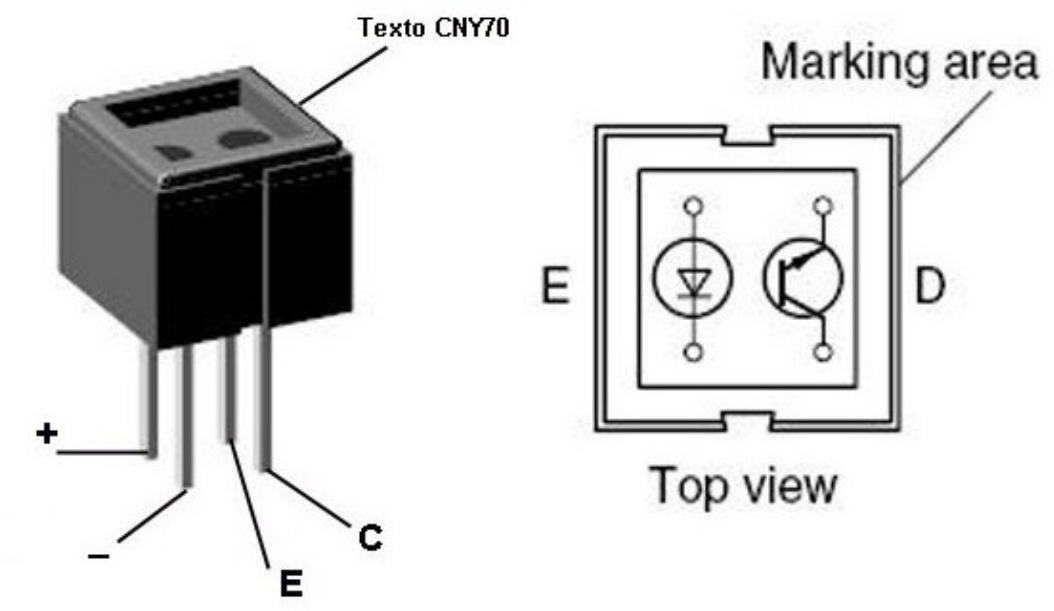
\includegraphics[width=.5\textwidth]{images/cny70}
 \caption{CNY 70}
 \label{fig:cny70}
\end{figure}

The CNY70 is a reflective optical sensor.
The emitter and the detector both use resistors to be polarized.
There is no clear formula for the detector as coupling factor varies with distance to the ground. Hence, we use trimmers to polarize the detector. 
Efficiency is a bit better with a polarization in the collector of the detector than in the emitter.

The CNY70 sensor make its detector current going up when the detector receive a light signal. To get a measure of this current, we use the voltage on the transistor's collector as shown on Figure~\ref{fig:cny70}.

\begin{figure}[!ht]
 \centering
 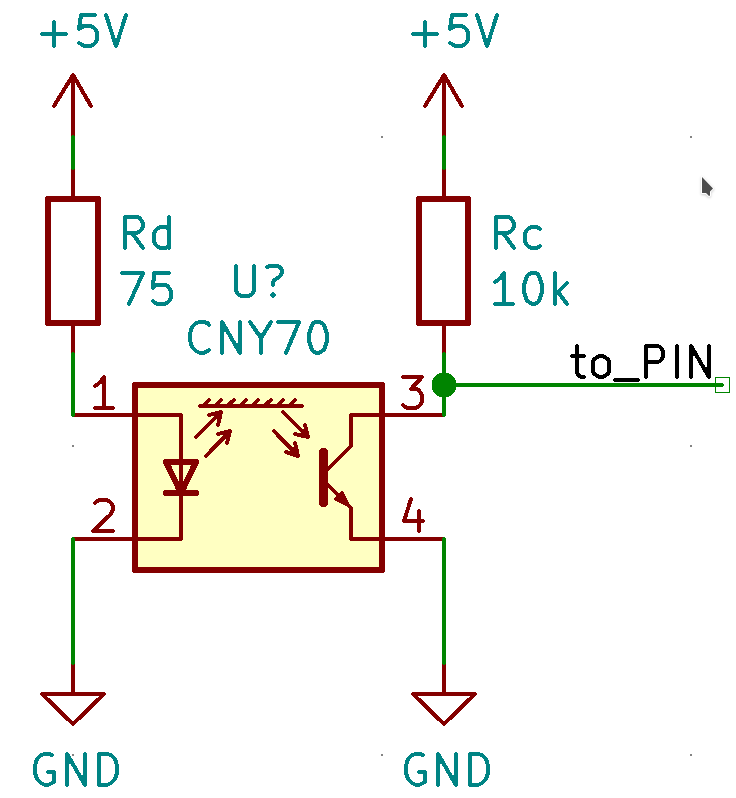
\includegraphics[width=.5\textwidth]{images/montage_cny}
 \caption{CNY 70 on the robot}
 \label{fig:cny70}
\end{figure}

\UPSTIremarque{When the detector is on a dark surface, the voltage \textit{to\_PIN} is \SI{5}{V}. \\
 When the detector is on a white surface, the voltage \textit{to\_PIN} is low t(around \SI{0}{V}).}

\subsection{Testing the CNY70 on the robot}

First, we need to identify the PIN linked to each sensor. The three sensors are connected on pins \textbf{PA\_7}, \textbf{PC\_2} and \textbf{PC\_3}.
Since we need to measure the voltage on each pin, they need to be configured as Analog inputs.

\inputminted[firstline=44, lastline=53]{C}{programmes/main.cpp}


\begin{UPSTIactivite}[][Get the CNY70 voltage][][][To do]
 \begin{enumerate}
  \item Edit the \mintinline{C}{includes/pin_connexions.h} file to \textbf{declare the sensors:}
        \begin{itemize}
         \item \mintinline{C}{cny_1} has already been declared : \mintinline{C}{DigitalIn cny_1 (PA_7);}
         \item Declare and connect \mintinline{C}{cny_2} to \textbf{PC\_2}
         \item Declare and connect \mintinline{C}{cny_3} to  \textbf{PC\_3}
        \end{itemize}
  \item Edit the \mintinline{C}{main.cpp} file to match the above code.
  \item Implement the function \mintinline{C}{ft_print_cny_analog_voltage(AnalogIn &analof_input, Serial pc)} in file \mintinline{C}{src/test_cny/ft_print_value_cny.cpp} :
        \begin{enumerate}
         \item Declare \mintinline{C}{value} and \mintinline{C}{voltage} variables (\mintinline{C}{double})
         \item Use the function \mintinline{C}{analog_input.read()} to get the converted analog value of the \mintinline{C}{analog_input} signal, put it in \mintinline{C}{value}.
         \item compute \mintinline{C}{voltage =  value * max_voltage;} to convert it.
         \item Use the \mintinline{C}{pc.printf("Voltage value : %lf ", voltage);} function to display the voltage value.
        \end{enumerate}
  \item Compile, download and transfer the executable file into the card.
  \item Identifie which sensor is connected to which signal.
        \begin{itemize}
         \item put a white sheet in front of each sensor and see which one react.
        \end{itemize}
 \end{enumerate}
\end{UPSTIactivite}
